% This LaTeX was auto-generated from MATLAB code.
% To make changes, update the MATLAB code and export to LaTeX again.

\documentclass{article}

\usepackage[utf8]{inputenc}
\usepackage[T1]{fontenc}
\usepackage{lmodern}
\usepackage{graphicx}
\usepackage{color}
\usepackage{hyperref}
\usepackage{amsmath}
\usepackage{amsfonts}
\usepackage{epstopdf}
\usepackage[table]{xcolor}
\usepackage{matlab}
\usepackage[paperheight=795pt,paperwidth=614pt,top=72pt,bottom=72pt,right=72pt,left=72pt,heightrounded]{geometry}

\sloppy
\epstopdfsetup{outdir=./}
\graphicspath{ {./ME419TermProj_Script_media/} }

\begin{document}

\matlabtitle{ME 419 Solar Tracking Panel Control Term Project }

\begin{par}
\begin{flushleft}
\textbf{Names:} Julia Fay, Aiden Taylor 
\end{flushleft}
\end{par}

\begin{par}
\begin{flushleft}
\textbf{Date:} 2024.3.20
\end{flushleft}
\end{par}

\begin{par}
\begin{flushleft}
\textbf{Class:} ME419
\end{flushleft}
\end{par}

\begin{par}
\begin{flushleft}
\textbf{Description: }The purpose of this file is to simulate the control of a solar tracking solar panel to compare to experimental behaviors found with testing. 
\end{flushleft}
\end{par}

\matlabheading{System Properties }

\begin{matlabcode}
% Visous damping coefficient 
b               = 10;               % [N*m*s/rad]
% Winding resistance
R               = 1;                % [Ω]
% Winding inductance
L               = 0.078e-3;         % [H]
% Rotor inertia
Jmotor          = 9.82e-7;          % [kg*m^2]
%Panel inertia 
Jpanel          = 5;                % [kg*m^2]
%Total inertia 
J               = Jmotor+Jpanel;    % [kg*m^2]
% Motor torque constant 
K_t             = 5;                % [N*m/A]
% Motor voltage constant 
K_v             = 5;                % [V*sec/rad]
% Radian to voltage conversion factor 
K_c             = 1/(0.5*pi());     % [V/rad]
\end{matlabcode}

\matlabheading{Block Diagram }

\begin{matlabcode}
snapshotModel('ME419TermProj') %output simulink image
\end{matlabcode}
\begin{center}
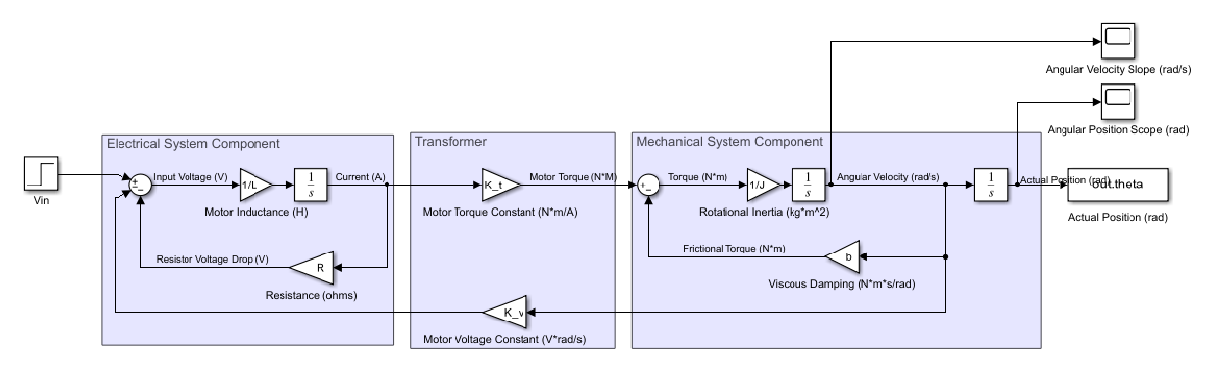
\includegraphics[width=\maxwidth{77.06974410436528em}]{figure_0.eps}
\end{center}

\matlabheading{Frictionless Simulation }

\begin{matlabcode}
%Input A,B,C, and K matricies 
b = 0;

K1 = [11.42 -121.01];

A_new_1 = [0              1
    -(K1(1,1))      -(((R*b + K_v^2)/R*J)+K1(1,2))];

B = [0
     1];

C = [((K_v*K_c)/R*J) 0];

D = [0];

sys1_tf = tf(((K_v*K_c)/R*J),[1 ((R*b + K_v^2)/R*J) 0])
\end{matlabcode}
\begin{matlaboutput}
sys1_tf =
 
     15.92
  -----------
  s^2 + 125 s
 
Continuous-time transfer function.
Model Properties
\end{matlaboutput}
\begin{matlabcode}

sys1 = ss(A_new_1,B,C,D);

figure; 
step(sys1)
xlabel("Time");
ylabel("Position (rad)");
title('Frictionless Panel and Motor Model Response to Step Input','FontSize',10,'FontWeight','bold');
grid on
\end{matlabcode}
\begin{center}
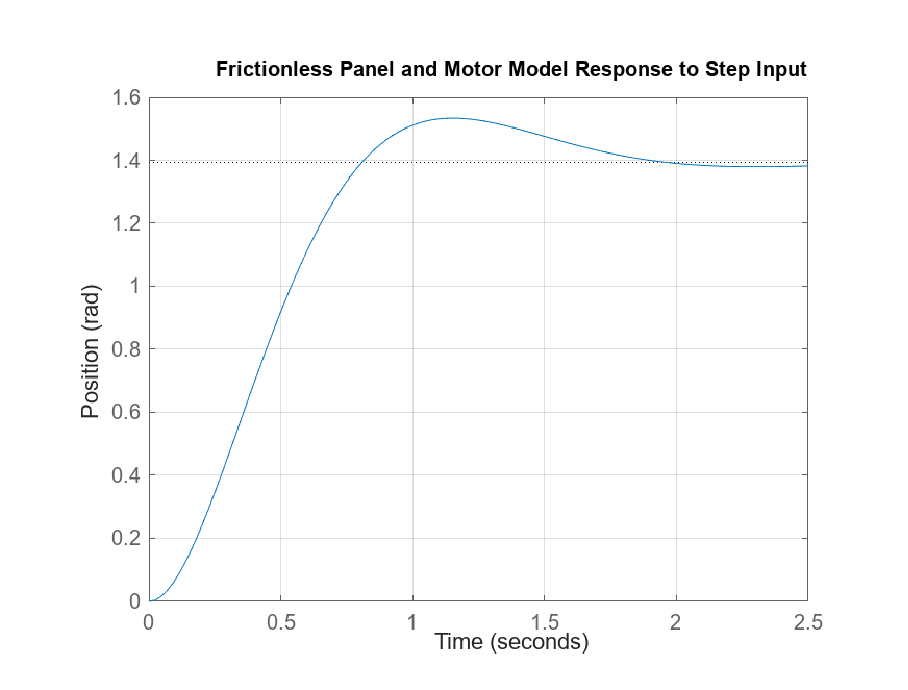
\includegraphics[width=\maxwidth{56.196688409433015em}]{figure_1.eps}
\end{center}
\begin{matlabcode}

%now try to simulate the system with friction using the K values calculated
%for the frictionless system
b = 10; 
K2 = [11.42 -121.01];

A_new_2 = [0              1
    -(K2(1,1))      -(((R*b + K_v^2)/R*J)+K2(1,2))];

sys2 = ss(A_new_2,B,C,D);
step(sys2)
xlabel("Time");
ylabel("Position (rad)");
title('Frictional Panel and Motor Model Step Response with Frictionless K Values','FontSize',10,'FontWeight','bold');
grid on
\end{matlabcode}
\begin{center}
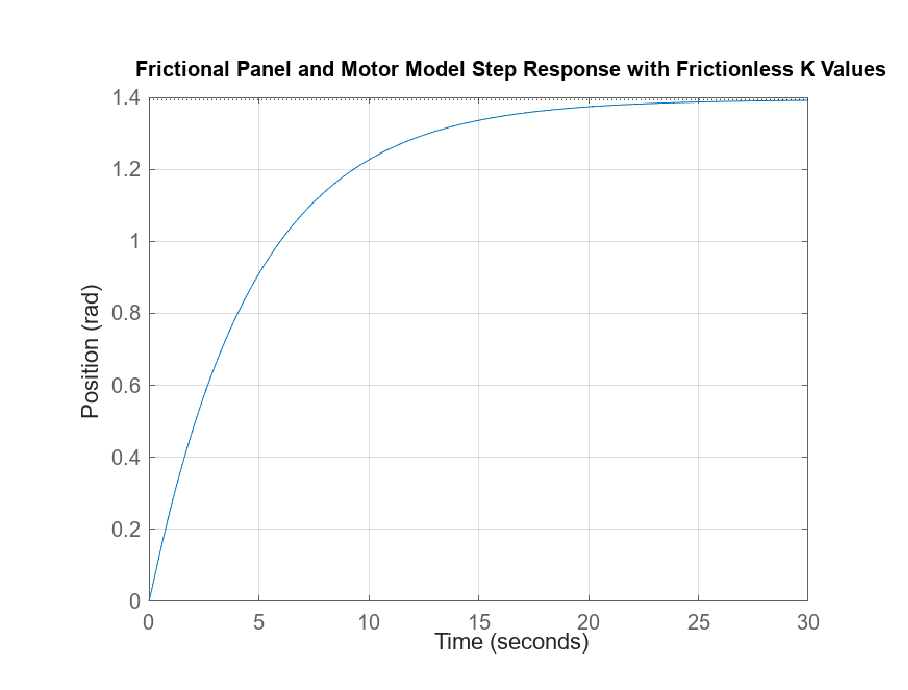
\includegraphics[width=\maxwidth{56.196688409433015em}]{figure_2.eps}
\end{center}

\matlabheading{Friction Simulation }

\begin{matlabcode}
%now reintroduce friction 
%Input Anew,B,C, and K matricies 
K3 = [11.42 -171.01];

A_new_3 = [0              1
    -(K3(1,1))      -(((R*b + K_v^2)/R*J)+K3(1,2))];

B1 = [0
     1];

C1 = [((K_v*K_c)/R*J) 0];

D1 = [0];

sys3_tf = tf(((K_v*K_c)/R*J),[1 ((R*b + K_v^2)/R*J) 0])
\end{matlabcode}
\begin{matlaboutput}
sys3_tf =
 
     15.92
  -----------
  s^2 + 175 s
 
Continuous-time transfer function.
Model Properties
\end{matlaboutput}
\begin{matlabcode}
sys3 = ss(A_new_3,B1,C1,D1);

figure; 
step(sys3)
xlabel("Time");
ylabel("Position (rad)");
title('Panel and Motor Model with Friction Response to Step Input','FontSize',10,'FontWeight','bold');
grid on
\end{matlabcode}
\begin{center}
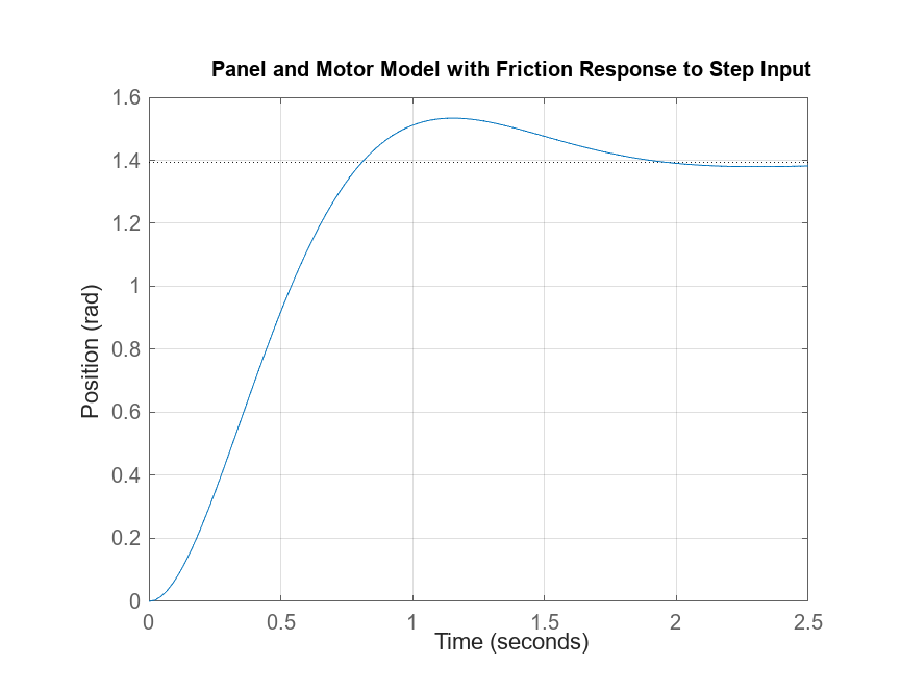
\includegraphics[width=\maxwidth{56.196688409433015em}]{figure_3.eps}
\end{center}

\end{document}
